\section{Local Optimization: Folding dan Simplification}

Optimasi lokal bekerja hanya di dalam satu \textit{basic block}. Tujuannya adalah mengurangi beban komputasi instruksi aritmatika tanpa perlu menganalisis seluruh program.

\subsection{1. Constant Folding}
Jika semua operan bersifat konstan, kompilator melakukan perhitungan saat itu juga.
\begin{itemize}
    \item \textbf{Sebelum}: \code{x = 2 * 3.14 * r}
    \item \textbf{Sesudah}: \code{x = 6.28 * r}
\end{itemize}

\subsection{2. Algebraic Simplification}
Menggunakan identitas matematika untuk menghapus operasi yang tidak perlu (\textit{Identity Elimination}).
\begin{itemize}
    \item \code{x + 0} $\to$ \code{x}
    \item \code{x * 1} $\to$ \code{x}
    \item \code{x / 1} $\to$ \code{x}
\end{itemize}

\subsection{3. Strength Reduction}
Mengganti operasi yang "mahal" (berat bagi CPU) dengan operasi yang "murah" namun ekuivalen. Biasanya dilakukan untuk perkalian dan pembagian dengan pangkat 2.
\begin{enumerate}
    \item \textbf{Multiplication}: \code{x * 2} diganti \code{x + x} atau \code{x << 1}.
    \item \textbf{Division}: \code{x / 4} diganti \code{x >> 2}.
    \item \textbf{Exponent}: \code{pow(x, 2)} diganti \code{x * x}.
\end{enumerate}

\begin{figure}[!htbp]
    \centering
    \adjustbox{max width=0.8\textwidth,center}{%
    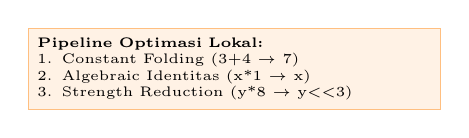
\begin{tikzpicture}[
        rect/.style={rectangle, draw=orange!50, fill=orange!10, text width=5cm, font=\tiny}
    ]
    \node[rect] (opt) {
        \textbf{Pipeline Optimasi Lokal:}\\
        1. Constant Folding (3+4 $\to$ 7)\\
        2. Algebraic Identitas (x*1 $\to$ x)\\
        3. Strength Reduction (y*8 $\to$ y<<3)
    };
    \end{tikzpicture}%
    }
    \caption{Hierarki Optimasi Lokal pada Ekspresi Aritmatika}
\end{figure}
